\documentclass[tikz,border=3pt]{standalone}
\usepackage{amsmath}
\usepackage{tikz}
\usetikzlibrary{arrows.meta}
\begin{document}
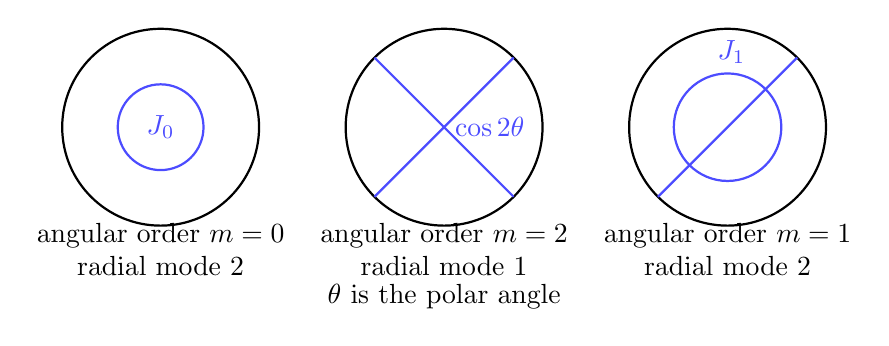
\begin{tikzpicture}[scale=1.0]
  \def\diskR{1.25}
  \def\jzeroring{0.5446} % 1.25*j_{0,1}/j_{0,2}
  \def\jonering{0.6827}  % 1.25*j_{1,1}/j_{1,2}
  \begin{scope}
    \draw[thick] (0,0) circle (\diskR);
    \draw[blue!70,thick] (0,0) circle (\jzeroring);
    \node[align=center] at (0,-1.55) {angular order $m=0$\\radial mode $2$};
    \node[blue!70] at (0,0) {$J_0$};
  \end{scope}
  \begin{scope}[xshift=3.6cm]
    \draw[thick] (0,0) circle (\diskR);
    \draw[blue!70,thick] ({-\diskR*cos(45)},{-\diskR*sin(45)}) -- ({\diskR*cos(45)},{\diskR*sin(45)});
    \draw[blue!70,thick] ({-\diskR*cos(45)},{\diskR*sin(45)}) -- ({\diskR*cos(45)},{-\diskR*sin(45)});
    \node[align=center] at (0,-1.55) {angular order $m=2$\\radial mode $1$};
    \node[blue!70] at (0.58,0.0) {$\cos 2\theta$};
  \end{scope}
  \begin{scope}[xshift=7.2cm]
    \draw[thick] (0,0) circle (\diskR);
    \draw[blue!70,thick] (0,0) circle (\jonering);
    \draw[blue!70,thick] ({-\diskR*cos(45)},{-\diskR*sin(45)}) -- ({\diskR*cos(45)},{\diskR*sin(45)});
    \node[align=center] at (0,-1.55) {angular order $m=1$\\radial mode $2$};
    \node[blue!70] at (0.05,0.95) {$J_1$};
  \end{scope}
  \node at (3.6,-2.15) {$\theta$ is the polar angle};
\end{tikzpicture}
\end{document}
